\documentclass[12pt]{article}
\usepackage[left=1cm, right=1cm, top=2cm,bottom=1.5cm]{geometry} 

\usepackage[parfill]{parskip}
\usepackage[utf8]{inputenc}
\usepackage[T2A]{fontenc}
\usepackage[russian]{babel}
\usepackage{enumitem}
\usepackage[normalem]{ulem}
\usepackage{amsfonts, amsmath, amsthm, amssymb, mathtools}
\usepackage{tabularx}
\usepackage{hhline}

\usepackage{accents}
\usepackage{fancyhdr}
\pagestyle{fancy}
\renewcommand{\headrulewidth}{1.5pt}
\renewcommand{\footrulewidth}{1pt}

\usepackage{graphicx}
\usepackage[figurename=Рис.]{caption}
\usepackage{subcaption}
\usepackage{float}

%%Наименование папки откуда забирать изображения
\graphicspath{ {./images/} }

%%Изменение формата для ввода доказательства
\renewcommand{\proofname}{$\square$  \nopunct}
\renewcommand\qedsymbol{$\blacksquare$}

%%Изменение отступа на таблицах
\addto\captionsrussian{%
	\renewcommand{\proofname}{$\square$ \nopunct}%
}
%% Римские цифры
\newcommand{\RN}[1]{%
	\textup{\uppercase\expandafter{\romannumeral#1}}%
}

%% Для удобства записи
\newcommand{\MR}{\mathbb{R}}
\newcommand{\MQ}{\mathbb{Q}}
\newcommand{\MN}{\mathbb{N}}
\newcommand{\MTB}{\mathbb{T}}
\newcommand{\MI}{\mathrm{I}}
\newcommand{\MJ}{\mathrm{J}}
\newcommand{\MH}{\mathrm{H}}
\newcommand{\MT}{\mathrm{T}}
\newcommand{\MU}{\mathcal{U}}
\newcommand{\MV}{\mathcal{V}}
\newcommand{\MW}{\mathcal{W}}
\newcommand{\VN}{\varnothing}
\newcommand{\VE}{\varepsilon}

\theoremstyle{definition}
\newtheorem{defn}{Опр:}
\newtheorem{rem}{Rm:}
\newtheorem{prop}{Утв.}
\newtheorem{exrc}{Упр.}
\newtheorem{lemma}{Лемма}
\newtheorem{theorem}{Теорема}
\newtheorem{corollary}{Следствие}

\newenvironment{cusdefn}[1]
{\renewcommand\thedefn{#1}\defn}
{\enddefn}

\DeclareRobustCommand{\divby}{%
	\mathrel{\text{\vbox{\baselineskip.65ex\lineskiplimit0pt\hbox{.}\hbox{.}\hbox{.}}}}%
}
%Короткий минус
\DeclareMathSymbol{\SMN}{\mathbin}{AMSa}{"39}
%Длинная шапка
\newcommand{\overbar}[1]{\mkern 1.5mu\overline{\mkern-1.5mu#1\mkern-1.5mu}\mkern 1.5mu}
%Функция знака
\DeclareMathOperator{\sgn}{sgn}

%Функция ранга
\DeclareMathOperator{\rk}{\text{rk}}

%Обозначение константы
\DeclareMathOperator{\const}{\text{const}}

%Интеграл в большом формате
\DeclareMathOperator{\dint}{\displaystyle\int}
\newcommand{\ddint}[2]{\displaystyle\int\limits_{#1}^{#2}}

\newcommand{\smallerrel}[1]{\mathrel{\mathpalette\smallerrelaux{#1}}}
\newcommand{\smallerrelaux}[2]{\raisebox{.1ex}{\scalebox{.75}{$#1#2$}}}

\newcommand{\smallin}{\smallerrel{\in}}
\newcommand{\smallnotin}{\smallerrel{\notin}}

\newcommand*{\medcap}{\mathbin{\scalebox{1.25}{\ensuremath{\cap}}}}%
\newcommand*{\medcup}{\mathbin{\scalebox{1.25}{\ensuremath{\cup}}}}%

\makeatletter
\newcommand{\vast}{\bBigg@{3.5}}
\newcommand{\Vast}{\bBigg@{5}}
\makeatother

%Скалярное произведение
\DeclarePairedDelimiterX{\inner}[2]{\langle}{\rangle}{#1, #2}

%Подпись символов снизу
\newcommand{\ubar}[1]{\underaccent{\bar}{#1}}

\begin{document}
\lhead{Математический анализ - \RN{2}}
\chead{Шапошников С.В.}
\rhead{Лекция - 21}
\section*{Мотивация интеграла Римана}
Ранее мы обсуждали неопределенные интегралы. Мы пришли к выводу, что кроме очень узкого класса функций первообразные найти (записав конечную формулу) очень трудно или почти невозможно. Возникает вопрос: как определять первообразные кроме алгебраического вычисления путем сведения к известным?

Пусть есть интервал $(a,b)$ и функция $f$. Мы хотим найти первообразную $F \colon F^\prime =f$. Пусть $F(x_0) = 0$, где $x_0 \in (a,b)$, хотим найти $F(x)$ в точке $x \in (a,b)$. Если $x$ и $x_0$ мало отличаются, то:
$$
	F(x) = F(x) - F(x_0) \approx F^\prime(x_0)(x - x_0) \Rightarrow F(x) \approx f(x_0)(x-x_0)
$$
Здесь ``примерно'' такое же, как и в определении дифференцируемости, то есть можно записать так:
$$
	F(x) = f(x_0)(x - x_0) + \overline{o}\big((x -  x_0)\big)
$$
Но нас интересуют значения функции $F$ не только рядом с точкой $x_0$, но вообще на интервале $(a,b)$.

\textbf{\uline{Идея}}: Умея на маленьких промежутках $[x_0,x_0 + \VE]$ хотя бы приблизительно указывать значения $F$, мы хотели бы научиться указывать значения на всем промежутке $[x_0, x]$.
\begin{figure}[H]
	\centering
	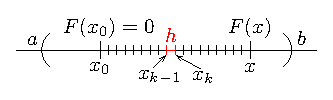
\includegraphics[width=0.35\textwidth]{21_1.eps}
	\caption{Нахождение значения функции $F$ в любой точке отрезка $[x_0,x]$.}
	\label{21_1}
\end{figure}
Разобьем промежуток $[x_0,x]$ точками $x_k$ и запишем $F(x)$ как сумму приращений на этих отрезках:
$$
	F(x) = \sum\limits_{k}\big(F(x_k) - F(x_{k-1})\big)
$$
Таким образом в сумме стоят приращения функции $F$ на маленьких отрезках. Пусть $x = x_N$, распишем эту сумму подробнее:
$$
	F(x) = F(x_N) - F(x_{N-1}) + F(x_{N-1}) - F(x_{N-2}) + \dotsc + F(x_1) - F(x_0) =  F(x_N) - F(x_0) = F(x_N) 
$$
Поскольку приращения маленькие, то каждое слагаемое в этой сумме можно заменить таким:
$$
	F(x) = \sum\limits_{k}\big(F(x_k) - F(x_{k-1})\big) = \sum\limits_{k}\Big(f(x_{k-1})(x_k - x_{k-1}) + \overline{o}\big((x_k - x_{k-1})\big) \Big)
$$
Если это $\overline{o}$ не зависит от отрезка на котором мы его рассматриваем:
$$
	\overline{o}\big((x_k - x_{k-1})\big) = \overline{o}(1){\cdot}(x_k - x_{k-1}), \, \lim\limits_{x_k \to x_{k-1}}\overline{o}(1) = \lim\limits_{h \to 0}\overline{o}(1) = 0, \, h = x_k - x_{k-1}, \, \forall k = \overline{1,N}
$$
и если мы можем его сделать единым для всех отрезков, то их сумма будет равна:
$$
	\sum\limits_k \overline{o}\big((x_k - x_{k-1})\big) = \overline{o}(1){\cdot} \sum\limits_k (x_k - x_{k-1}) = \overline{o}(1){\cdot}(x - x_0)
$$
Выбирая все больше точек разбиения и мельче отрезки разбиения, эта сумма устремится к нулю:
$$
	\lim\limits_{h \to 0}\overline{o}(1) = 0 \Rightarrow \lim\limits_{h \to 0}\sum\limits_k \overline{o}\big((x_k - x_{k-1})\big) = 0
$$
Следовательно функция $F(x)$ это в определенном смысле следующий предел:
$$
	F(x) = \lim\limits_{h \to 0}\sum\limits_{k}f(x_{k-1})(x_k - x_{k-1})
$$
\newpage
Чтобы избежать использования бесконечно малых, мы можем воспользоваться теоремой Лагранжа:
$$
	F(x) = \sum\limits_{k}\big(F(x_k) - F(x_{k-1})\big) = \sum\limits_{k}f(c_k)(x_k - x_{k-1}), \, c_k \in [x_{k-1}, x_k]
$$
Но тогда не ясно какие точки $c_k$ необходимо брать, теорема Лагранжа никакого конструктивного ответа как выбирать $c_k$ не дает. С другой стороны, если мы можем восстанавливать $F(x)$ таким способом, то наверное ответ не должен зависеть от выбора точки $c_k$. А если мы будем брать произвольные $c_k$, то возникнут бесконечно малые величиные ($\overline{o}$).

В результате, возникают вопросы: как правильно эту конструкцию формализовать, в каком смысле понимать здесь предел и для каких функций $f$ это сработает? На эти вопросы можно ответить используя интеграл Римана.

\section*{Интеграл Римана}
Пусть имеется отрезок $[a,b]$.
\begin{defn}
	\uwave{Разбиением} $\MTB$ на отрезке $[a,b]$ назовем набор точек: $\MTB = \{a = x_0 < x_1 < \dotsc < x_N = b\}$.
\end{defn}
\begin{defn}
	\uwave{Отрезками разбиения} $\MTB$ будем называть отрезки $\Delta_k$ такие, что: $$
		\Delta_k = [x_{k-1}, x_k], \, |\Delta_k| = x_k - x_{k-1}, \, k = \overline{1,N},\, \sum\limits_{k = 1}^N |\Delta_k| =  b - a
	$$
\end{defn}
\begin{defn}
	\uwave{Масштабом} или \uwave{параметром разбиения} $\lambda(\MTB)$ будем называть длину наибольшего отрезка разбиения:
	$$
		\lambda(\MTB) = \max\limits_{k}|\Delta_k|
	$$
\end{defn}
\begin{defn}
	\uwave{Отмеченным разбиением} будем называть пару $(\MTB,\xi)$, где $\xi = (\xi_1,\dotsc, \xi_N), \, \xi_k \in \Delta_k$ - набор точек.
\end{defn}
\begin{rem}
	Проще говоря, отмеченное разбиение это выбранные в каждом отрезке разбиения точки (говорят отмеченные точки).
\end{rem}
\begin{figure}[H]
	\centering
	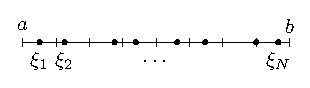
\includegraphics[width=0.3\textwidth]{21_2.eps}
	\caption{Отмеченное разбиение $(\MTB, \xi)$.}
	\label{21_2}
\end{figure}
Пусть на $[a,b]$ задана функция $f$.
\begin{defn}
	\uwave{Римановой суммой} называется сумма $\sigma(f, \MTB, \xi) = \displaystyle \sum\limits_{k = 1}^{N}f(\xi_k){\cdot}|\Delta_k| = f(\xi_1){\cdot}|\Delta_1| + \dotsc + f(\xi_N){\cdot}|\Delta_N|$.
\end{defn}
Риманова сумма по форме это ровно то, что мы писали ранее для восстановления первообразной. Но помимо этого, она несёт в себе достатчно простой геометрический смысл.

\textbf{\uline{Геометрический смысл}}: Риманова сумма представляет из себя сумму площадей прямоугольников, которая приближается к площади подграфика.
\begin{figure}[H]
	\centering
	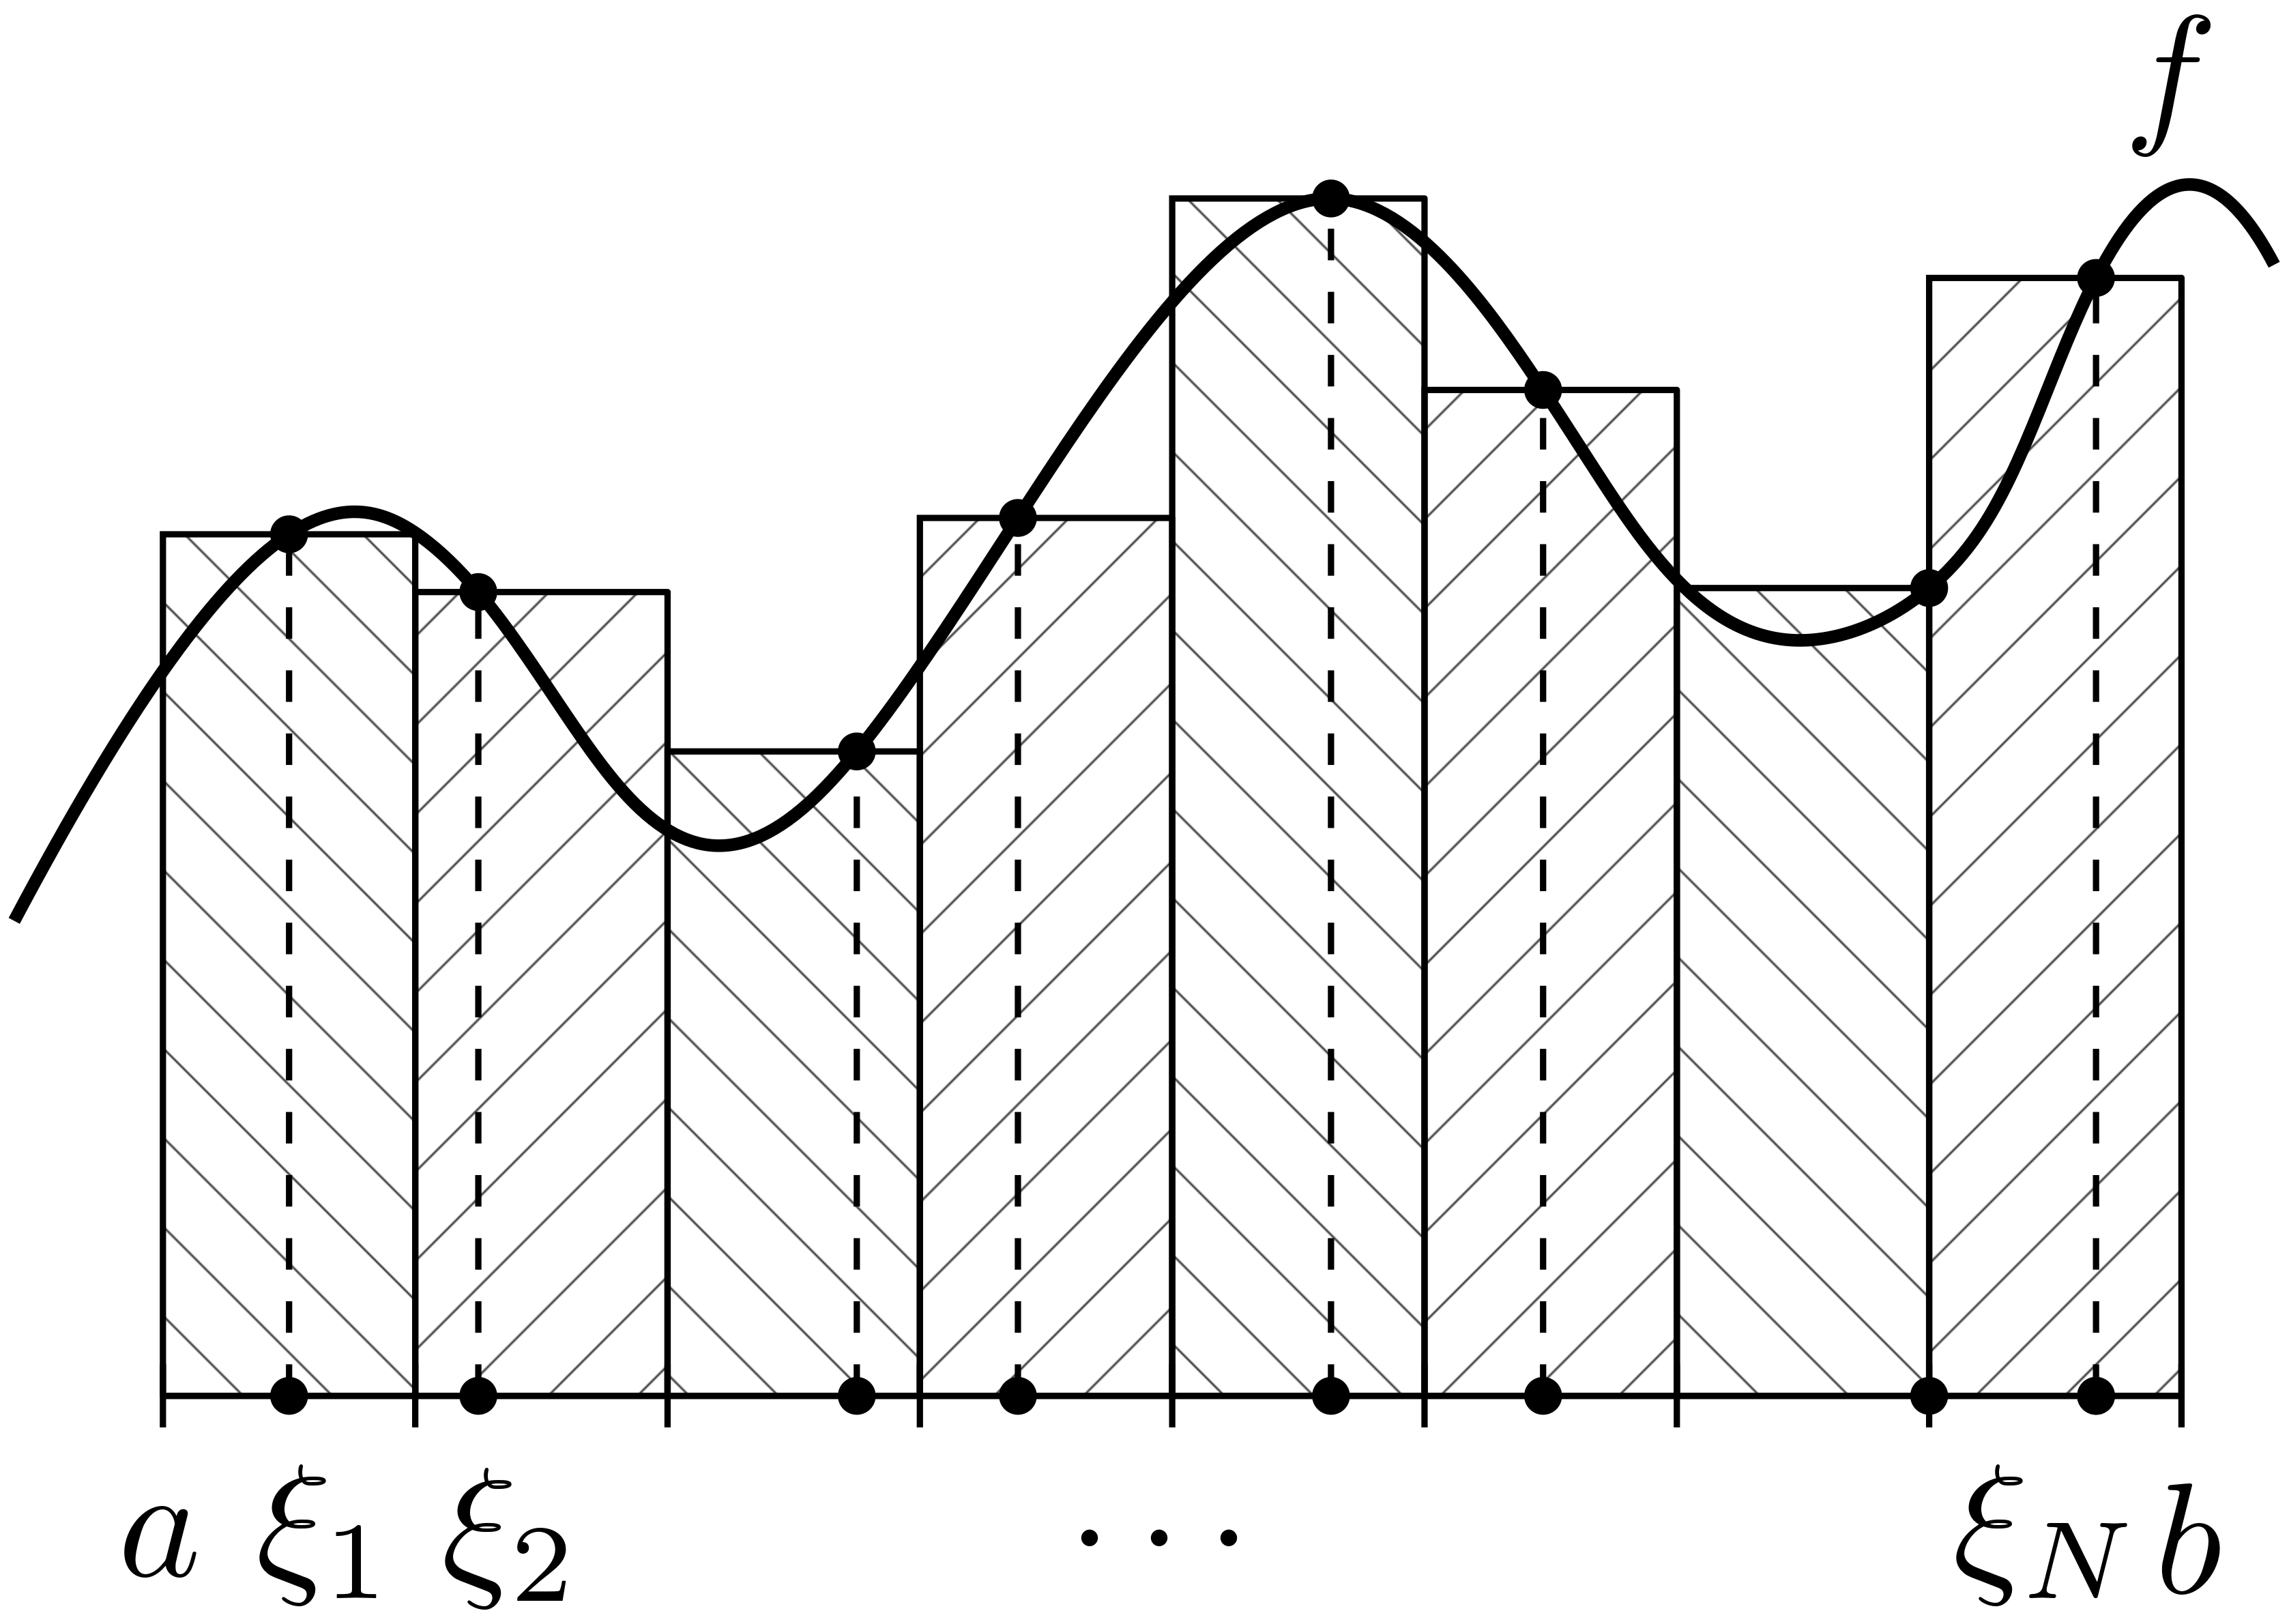
\includegraphics[width=0.4\textwidth]{21_3.png}
	\caption{Риманова сумма $\sigma(f, \MTB, \xi)$ для функции $f$ как сумма площадей прямоугольников.}
	\label{21_3}
\end{figure}
\begin{defn}
	Функция $f$ \uwave{интегрируема по Риману} на отрезке $[a,b]$ и число $\MI$ - её \uwave{интеграл}, если:
	$$
		\forall \VE > 0,\, \exists \, \delta > 0 \colon \forall (\MTB, \xi), \, \lambda(\MTB) < \delta \Rightarrow |\sigma(f, \MTB, \xi) - \MI| < \VE
	$$
	Число $\MI$ прянято называть \uwave{определенным интегралом} и обозначать следующим образом: 
	$$
		\MI = \ddint{a}{b}f(x)dx
	$$
\end{defn}
\begin{rem}
	Определение должно напоминать определение предела, но здесь нет единственного параметра, который куда-то стремится. Например, при каждом значении параметра может быть сколь угодно много отмеченных разбиений, удовлетворяющих свойству $\lambda(\MTB) < \delta$.
\end{rem}
\begin{rem}
	Также заметим, что никаких ограничений на $\xi$ нет, то есть отмеченные точки могут быть какими угодно в отрезках разбиения.
\end{rem}
На самом деле интегрируемость по Риману может быть записана на языке пределов по базе.
\subsection*{Интеграл Римана как предел по базе}
Вспомним определение из предыдущего семестра. Пусть $X \neq \varnothing$.
\begin{defn}
	\uwave{Базой} называется такой непустой набор $\mathfrak{B}$ подмножеств $X$, что 
	\begin{enumerate}[label={(\arabic*)}]
		\item $\varnothing \notin \mathfrak{B}$;
		\item $\forall B_1, B_2 \in \mathcal{B},\, \exists \, B_3 \in \mathfrak{B} \colon B_3 \subset B_1 \cap B_2$;
	\end{enumerate}
\end{defn}
\begin{defn}
	Число $A = \lim\limits_{\mathcal{B}}f$ называется \uwave{пределом} $f$ \uwave{по базе} $\mathfrak{B}$, если:
	$$
		\forall \varepsilon > 0, \, \exists \, B \in \mathfrak{B} \colon \forall x \in B, \, |f(x) - A| < \varepsilon
	$$ 
\end{defn}
Пусть $X = \{(\MTB, \xi)\}$ - множество всех возможных разбиений. В качестве элементов базы возьмем всевозможные наборы $B_\delta$, где $B_\delta$ это все разбиения масштаб которых меньше $\delta$: 
$$
	\mathfrak{B} = \{B_\delta\}, \, B_\delta = \{(\MTB, \xi)\mid \lambda(\MTB) < \delta \}, \, \delta > 0
$$
\begin{prop}
	Заданное таким образом множество $\mathfrak{B}$ является базой.
\end{prop}
\begin{proof}
	Проверим по определению, что $\mathfrak{B}$ - база:
	\begin{enumerate}[label={(\arabic*)}]
		\item Какое бы малое $\delta > 0$ мы не задали, всегда можно разбить отрезок таким образом, что шаг будет меньше $\delta \Rightarrow \VN \notin \mathfrak{B}$;
		\item $\forall B_{\delta_1}, B_{\delta_2} \in \mathfrak{B},\, \exists \, B_{\min\{\delta_1,\delta_2\}} \in \mathfrak{B} \colon B_{\min\{\delta_1,\delta_2\}} \subset B_{\delta_1} \cap B_{\delta_2}$;
	\end{enumerate}
\end{proof}
\begin{rem}
	Обычно вместо предела по базе $\mathfrak{B}$ пишут предел при $\lambda(\MTB) \to 0$, понимая что это описывается как предел по базе.
\end{rem}
Тогда, определенный интеграл Римана от $a$ до $b$ функции $f$ это просто предел по заданной базе:
$$
	\ddint{a}{b}f(x)dx = \lim\limits_{\mathfrak{B}}\sigma(f, \MTB, \xi) = \lim\limits_{\lambda(\MTB) \to 0}\sigma(f, \MTB, \xi)
$$
Или строго по определению:
$$
	\forall \VE > 0, \, \exists B_\delta \colon \forall (\MTB, \xi) \in B_\delta \Rightarrow \left|\sigma(f, \MTB, \xi) - \ddint{a}{b}f(x)dx\right| < \VE
$$
Отметим, что можно было бы взять все свойства предела по базе и переформулировать их как свойства интеграла Римана: арифметика пределов, переход к пределам в неравенствах, единственность пределов, критерий Коши (не обсуждали) и так далее. Мы лишь отметим что из этого следует единственность пределов $\Rightarrow$ единственность интегралов Римана.

\subsection*{Примеры определенных интегралов}
\begin{enumerate}[label={\arabic*)}]
	\item $f(x) \equiv 1$, по определению: $\sigma(f, \MTB, \xi) = \displaystyle \sum\limits_{k = 1}^{N}f(\xi_k){\cdot}|\Delta_k| =  \displaystyle \sum\limits_{k = 1}^{N}|\Delta_k| = b -a \Rightarrow \ddint{a}{b}1{\cdot}dx = b-a$; 
	\item $f(x) = \mathcal{D}(x)= 
	\begin{cases} 
		1, & x \in \mathbb{Q} \\
		0, & x \notin \mathbb{Q} 
	\end{cases}$ - функция Дирихле. Если $\xi_k \in \MQ$, то $\sigma(f, \MTB, \xi) = b - a$. Если же $\xi_k \notin \MQ$, то $\sigma(f, \MTB, \xi) = 0$. Получается что эта функция не интегрируема. 

	Пусть это не так и функция интегрируема, тогда в малом масштабе разбиения будет верно: 
	$$
		|\sigma - A| < \dfrac{b-a}{2}
	$$ 
	Но это бы одновременно означало, что $b-a$ отлично от $A$ на меньше, чем $\tfrac{b-a}{2}$ и $0$ отличен от $A$ на эту же величину $\Rightarrow$ нет такого предела $\Rightarrow$ функция Дирихле не является интегрируемой;
	\item $f(x) = \mathbb{I}_J(x)= 
	\begin{cases} 
		1, & x \in J \\
		0, & x \notin J 
	\end{cases}$, где $J \in [a,b]$ - это промежуток с концами $c \leq d$, где $a \leq c \leq d \leq b$.
	\begin{prop}
		Функция $f(x) = \mathbb{I}_J(x)$ интегрируема на $[a,b]$ и $\ddint{a}{b}f(x)dx = d - c$.
	\end{prop}
	\begin{proof}
		Точки $c$ и $d$ могут находиться внутри отрезка разбиения или быть на одном из концов такого отрезка (то есть $c$ или $d$ это какой-то $x_k$ разбиения).
		Следовательно, все множество отрезков $\{\Delta_k\}$ мы можем разбить на три группы:
		\begin{enumerate}[label={(\Roman*)}]
			\item Отрезки содержащие $c$ и $d$. Поскольку обе точки могут лежать на концах отрезков, то их число будет не больше $4$;
			\item Отрезки внутри интервала $(c,d)$;
			\item Отрезки в дополнении к $[c,d]$;
		\end{enumerate}
		Эти три группы не пересекаются и $\{\Delta_k\} = (\RN{1}) \sqcup (\RN{2}) \sqcup (\RN{3})$. Построим Риманову сумму:
		$$
			\sigma(f, \MTB, \xi) = \displaystyle \sum\limits_{k = 1}^{N}f(\xi_k){\cdot}|\Delta_k| = \displaystyle \sum\limits_{k \colon \Delta_k \in (\RN{1})}f(\xi_k){\cdot}|\Delta_k| + \displaystyle \sum\limits_{k \colon \Delta_k \in (\RN{2})}f(\xi_k){\cdot}|\Delta_k| + \displaystyle \sum\limits_{k \colon \Delta_k \in (\RN{3})}f(\xi_k){\cdot}|\Delta_k| = 
		$$
		$$
			= \underbrace{\displaystyle \sum\limits_{k \colon \Delta_k \in (\RN{1})}f(\xi_k){\cdot}|\Delta_k|}_{ \geq 0} + \displaystyle \sum\limits_{k \colon \Delta_k \subset (c,d)}f(\xi_k){\cdot}|\Delta_k| + 0 = \displaystyle \sum\limits_{k \colon \Delta_k \in (\RN{1})}f(\xi_k){\cdot}|\Delta_k + \displaystyle \sum\limits_{k \colon \Delta_k \subset (c,d)}|\Delta_k|
		$$
		Поскольку отрезков из группы $(\RN{1})$ не больше $4$, то:
		$$
			0 \leq \displaystyle \sum\limits_{k \colon \Delta_k \in (\RN{1})}f(\xi_k){\cdot}|\Delta_k| \leq 4 \lambda(\MTB)
		$$
		Сумма длин отрезков внутри интервала $(c,d)$ заведомо не больше, чем $d - c$. Эта же сумма отличается от $d-c$ не больше, чем на сумму длин интервалов покрывающих $c$ и $d$, то есть $2\lambda(\MTB)$:
		$$
			d-c - 2 \lambda(\MTB) \leq \displaystyle \sum\limits_{k \colon \Delta_k \subset (c,d)}|\Delta_k| \leq d - c
		$$
		\begin{figure}[H]
			\centering
			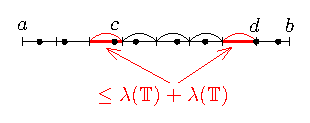
\includegraphics[width=0.3\textwidth]{21_4.eps}
			\caption{Отрезки покрывающие $c$ и $d$ рядом с интервалом $(c,d)$.}
			\label{21_4}
		\end{figure}
		Подводя итог, мы получаем:
		$$
			 -2 \lambda(\MTB) \leq \sigma(f, \MTB, \xi) - (d - c)  \leq 4 \lambda(\MTB)
		$$
		По определению:
		$$
			\forall \VE > 0, \, \delta = \dfrac{\VE}{4} > 0, \, \forall (\MTB, \xi), \lambda(\MTB) < \delta \Rightarrow |\sigma(f, \MTB, \xi) - (d - c)| \leq 4 \lambda(\MTB) < 4 \delta < \VE
		$$
	\end{proof}
\end{enumerate}
\section*{Свойства интеграла Римана}
Почти все свойства интеграла Римана будут унаследованы от пределов.

$1)$ \textbf{(\uline{Линейность})}: Если $f$ и $g$ интегрируемы по Риману на $[a,b]$, то $\forall \alpha, \beta \in \MR$ функция $\alpha{\cdot}f + \beta{\cdot}g$ интегрируема по Риману и верно:
$$
	\ddint{a}{b}(\alpha {\cdot} f + \beta {\cdot} g) dx = \alpha \ddint{a}{b}fdx + \beta\ddint{a}{b}gdx
$$
\begin{proof}
	Рассмотрим сразу $\delta > 0$ общее для $f$ и $g$ (взяли минимальное из $\delta_f, \delta_g$):
	$$
		\forall \VE > 0, \, \exists \, \delta > 0 \colon \forall (\MTB, \xi),\, \lambda(\MTB) \Rightarrow \left|\ddint{a}{b}fdx - \sigma(f, \MTB,\xi)\right| < \VE \wedge \left|\ddint{a}{b}gdx - \sigma(g, \MTB,\xi)\right| < \VE
	$$
	Заметим что по определению Римановой суммы: 
	$$
		\sigma(\alpha {\cdot} f + \beta {\cdot} g, \MTB, \xi) = \alpha{\cdot} \sigma(f, \MTB,\xi) + \beta{\cdot}\sigma(g, \MTB,\xi)
	$$ 
	Оценим следующую разность через неравенство треугольника:
	$$
		\left|\alpha\ddint{a}{b}fdx + \beta\ddint{a}{b}gdx - \sigma(\alpha {\cdot} f + \beta {\cdot} g, \MTB, \xi)\right| \leq |\alpha|{\cdot}\left| \ddint{a}{b}fdx - \sigma(f, \MTB,\xi)\right| + |\beta|{\cdot}\left|\ddint{a}{b}gdx - \sigma(g, \MTB,\xi)\right| \leq C \VE
	$$
	где $C = |\alpha| + |\beta|$, но константа при всяком $\VE$ не важна.
\end{proof}
\begin{corollary}
	Пусть $J_1,\dotsc, J_M$ - любые промежутки в отрезке $[a,b]$. Следующая функция:
	$$
		f(x) = \displaystyle \sum\limits_{m=1}^Mc_m{\cdot}\mathbb{I}_{J_m}(x)
	$$ 
	интегрируема по Риману и её интеграл равен:
	$$
		\ddint{a}{b}f(x)dx = \displaystyle \sum\limits_{m=1}^Mc_m{\cdot}|J_m|
	$$
\end{corollary}
\begin{proof}
	Следует сразу же из примера выше и линейности.
\end{proof}
$2)$ \textbf{(\uline{Монотонность})}: Если $f$ и $g$ интегрируемы на $[a,b]$ и $f \leq g$ на $[a,b]$, то верно:
$$
	\ddint{a}{b}f(x)dx \leq \ddint{a}{b}g(x)dx
$$
\begin{proof}
	Достаточно доказать для $f \equiv 0$, так как:
	$$
		\ddint{a}{b}f(x)dx \leq \ddint{a}{b}g(x)dx \Leftrightarrow 0 \leq \ddint{a}{b}\big(g(x) - f(x)\big)dx 
	$$
	Покажем, что если $g \geq 0$, то $\ddint{a}{b}g(x)dx \geq 0$. По определению интеграла Римана:
	$$
		\forall \VE > 0, \, \exists \, \delta > 0 \colon \forall (\MTB, \xi), \, \lambda(\MTB) < \delta \Rightarrow \ddint{a}{b}gdx \geq \sigma(g,\MTB,\xi) - \VE \geq 0 - \VE = - \VE \Rightarrow \VE \to 0 \Rightarrow \ddint{a}{b}g(x)dx \geq 0
	$$
	где $\sigma(g,\MTB,\xi) = \displaystyle \sum\limits_{k = 1}^{N}g(\xi_k){\cdot}|\Delta_k| \geq 0$, так как $g(x) \geq 0, \, \forall x \in [a,b]$.
\end{proof}

\begin{corollary}\textbf{(Теорема о среднем)}
	Пусть $f$ интегрируема на отрезке $[a,b]$ и $m \leq f \leq M$, тогда $\exists \, \mu \in [m,M]$ такая, что:
	$$
		\ddint{a}{b}f(x)dx = \mu{\cdot}(b-a)	
	$$
	Более того, если $f \in C[a,b]$, то $\mu = f(c)$ для некоторого $c \in [a,b]$.
\end{corollary}

\textbf{\uline{Геометрический смысл}}: Интеграл Римана несет в себе смысл площади под графиком функции. Теорема говорит о том, что между минимальным и максимальным значением функции $f$ найдется такое значение $f(c) = \mu$, что если проведём линию $y = \mu$ и возьмем площадь прямоугольника под этой линией на отрезке $[a,b]$, то она будет такой же, как и площадь под графиком $f$.
\begin{figure}[H]
	\centering
	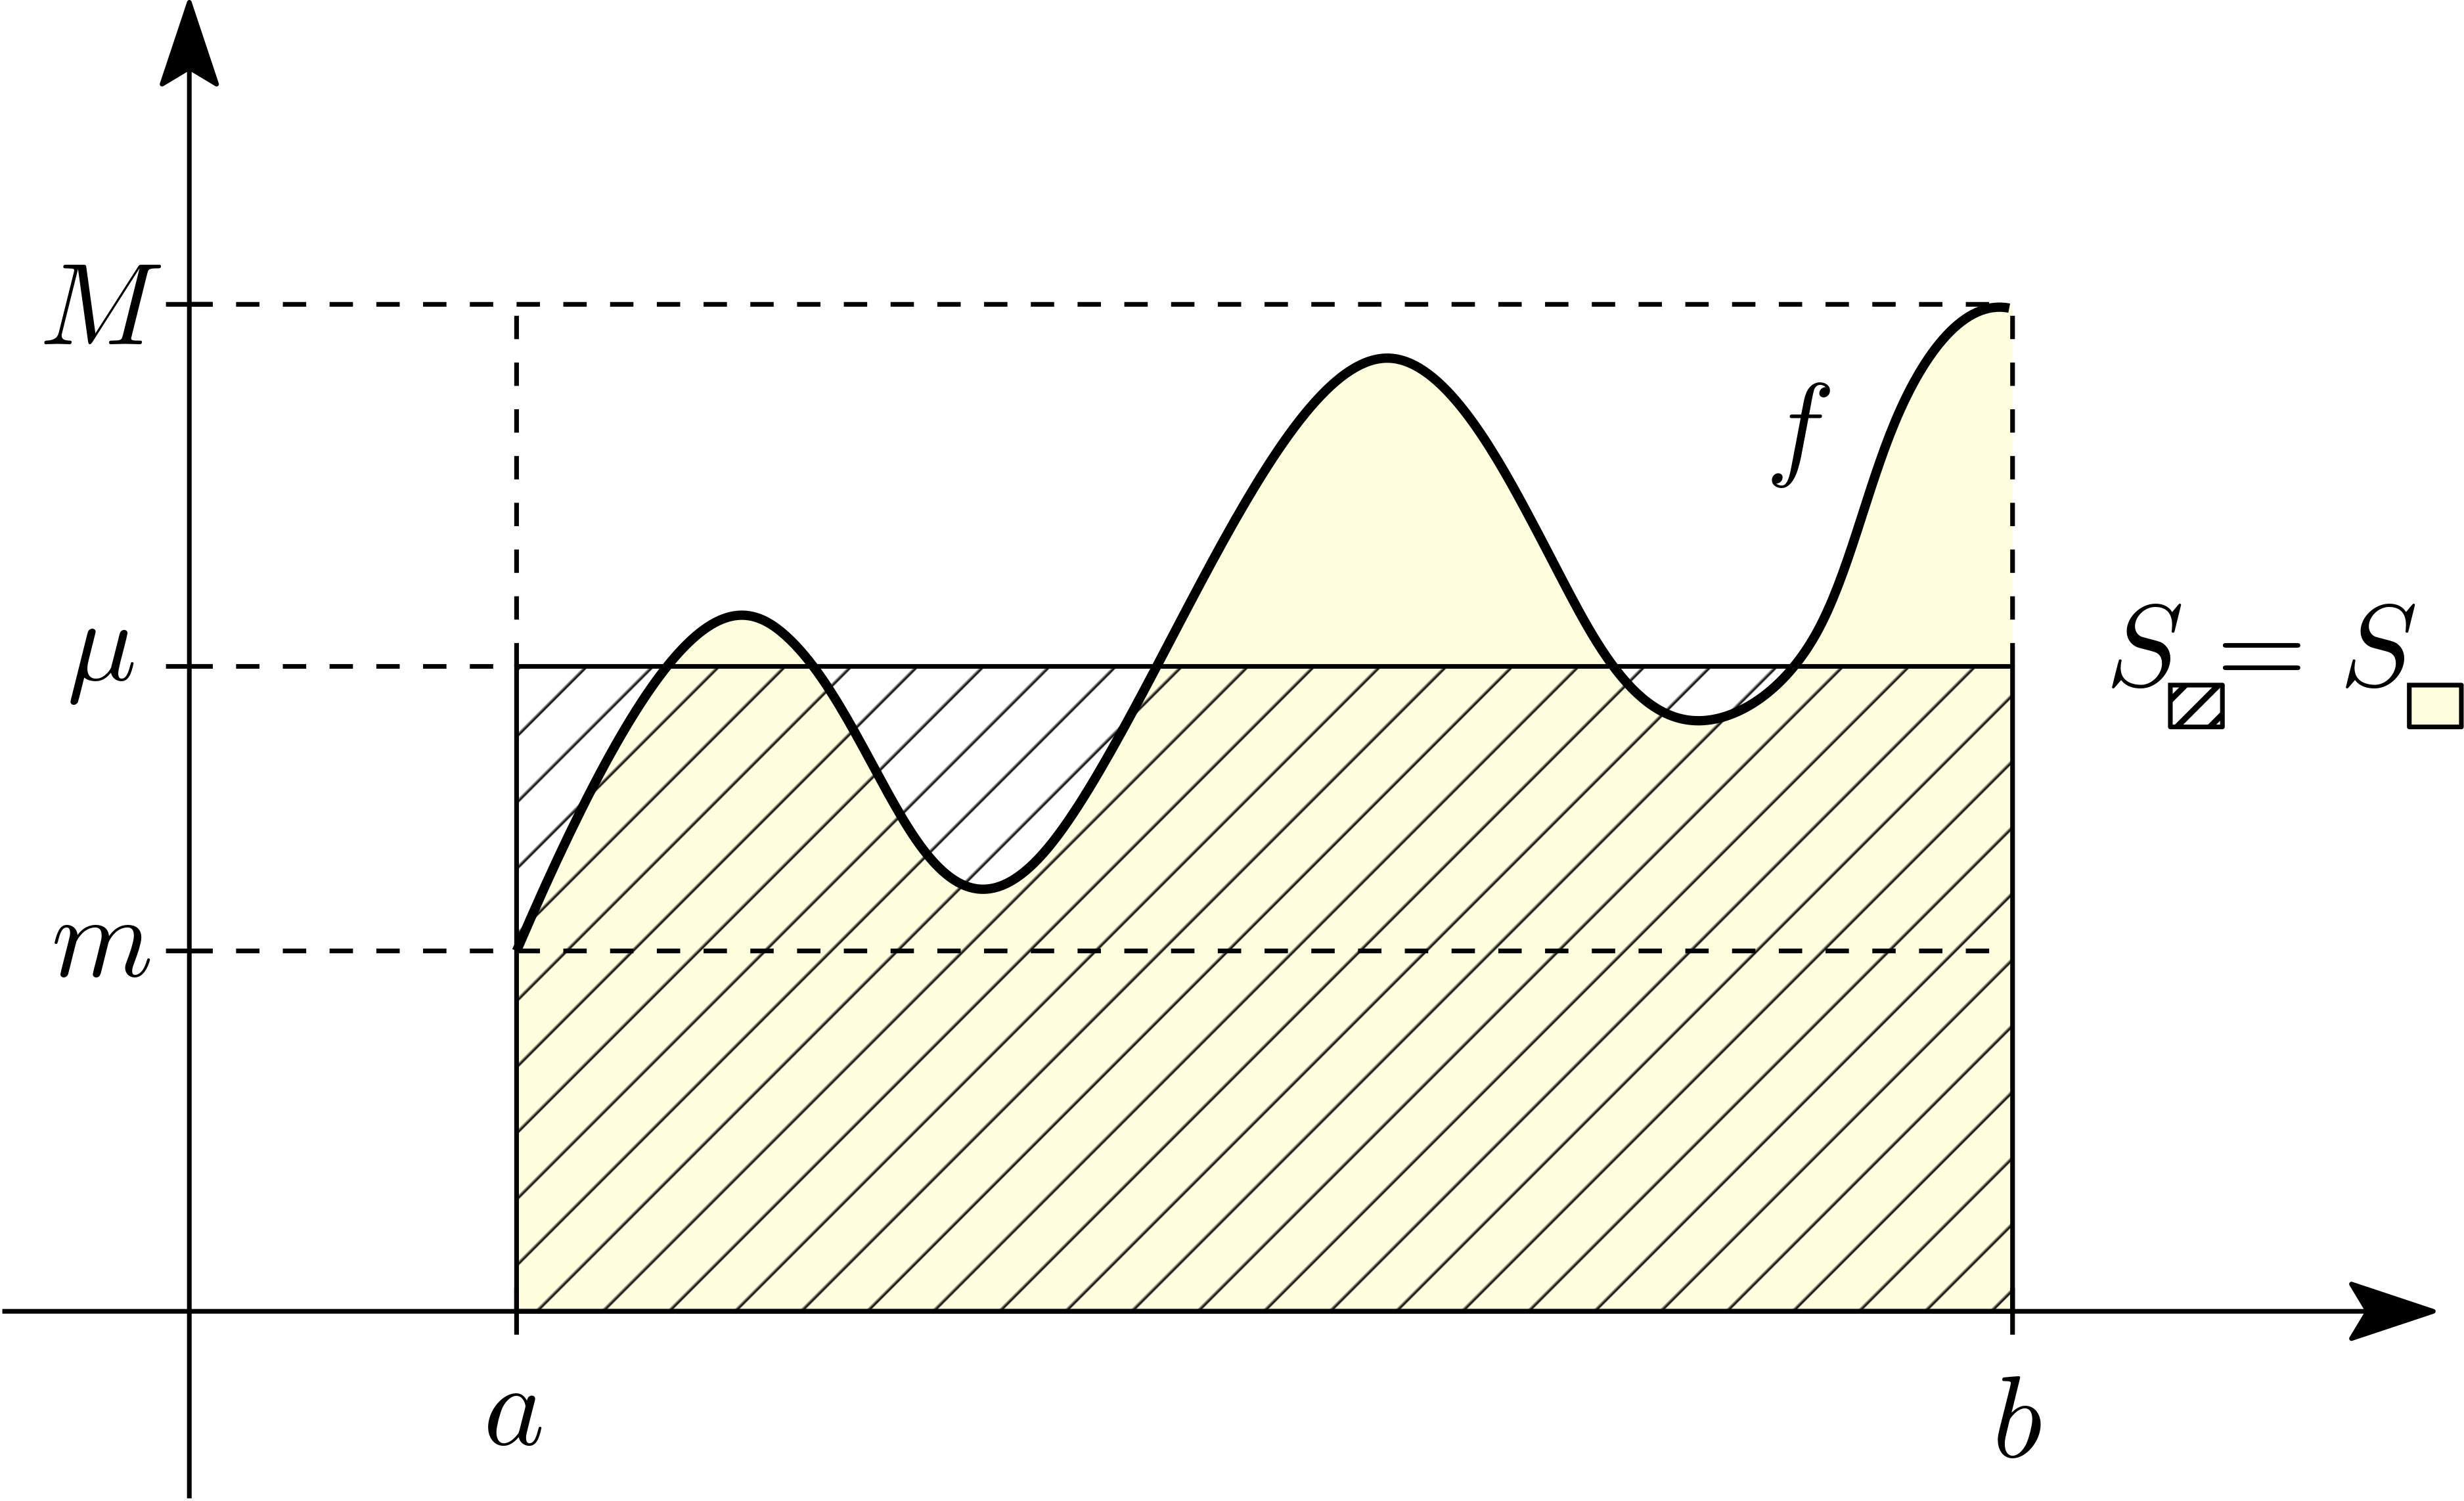
\includegraphics[width=0.6\textwidth]{21_5.png}
	\caption{Геометрический смысл теоремы о среднем.}
	\label{21_5}
\end{figure}
Или что то же самое, площадь под графиком можно заменить площадью прямоугольника выбрав в качестве высоты некоторое значение между минимумом и максимумом функции $f$.
\begin{proof}
	Из неравенств $m \leq f(x) \leq M$ перейдем в интегралы, где по монотонности:
	$$
		m{\cdot}(b-a) = \ddint{a}{b}m{\cdot}dx \leq \ddint{a}{b}f(x)dx \leq \ddint{a}{b}M{\cdot}dx = M{\cdot}(b-a)
	$$
	Разделим на $(b-a) > 0$ - положительное число, получим:
	$$
		m \leq \dfrac{1}{b-a}\ddint{a}{b}f(x)dx \leq M
	$$
	отсюда возьмем $\mu = \dfrac{1}{b-a}\ddint{a}{b}f(x)dx \Rightarrow (b-a){\cdot}\mu = \ddint{a}{b}f(x)dx$ и $m \leq \mu \leq M$.
	
	Если функция $f \in C[a,b]$, то можно взять $m = \min\limits_{[a,b]}f$ и $M = \max\limits_{[a,b]}f$, которые по теореме Вейрштрасса достигаются. Следовательно, по теореме о промежуточном значении $\exists \, c \in [a,b] \colon \mu = f(c)$.
\end{proof}
\end{document}